\chapter{Installation of AOM}\label{AOMInstallChapter}

We generate shifted beams by sending the seed light through an Acousto-optic Modulator (AOM)\footnote{also known as an Acousto-optic frequency shifter} using a double pass configuration. This is illustrated in Figure\,\ref{aomDiagramDetail}. A photograph of the AOM can be seen in Figure\,\ref{aom_upclose}.

\begin{figure}
\centerline{
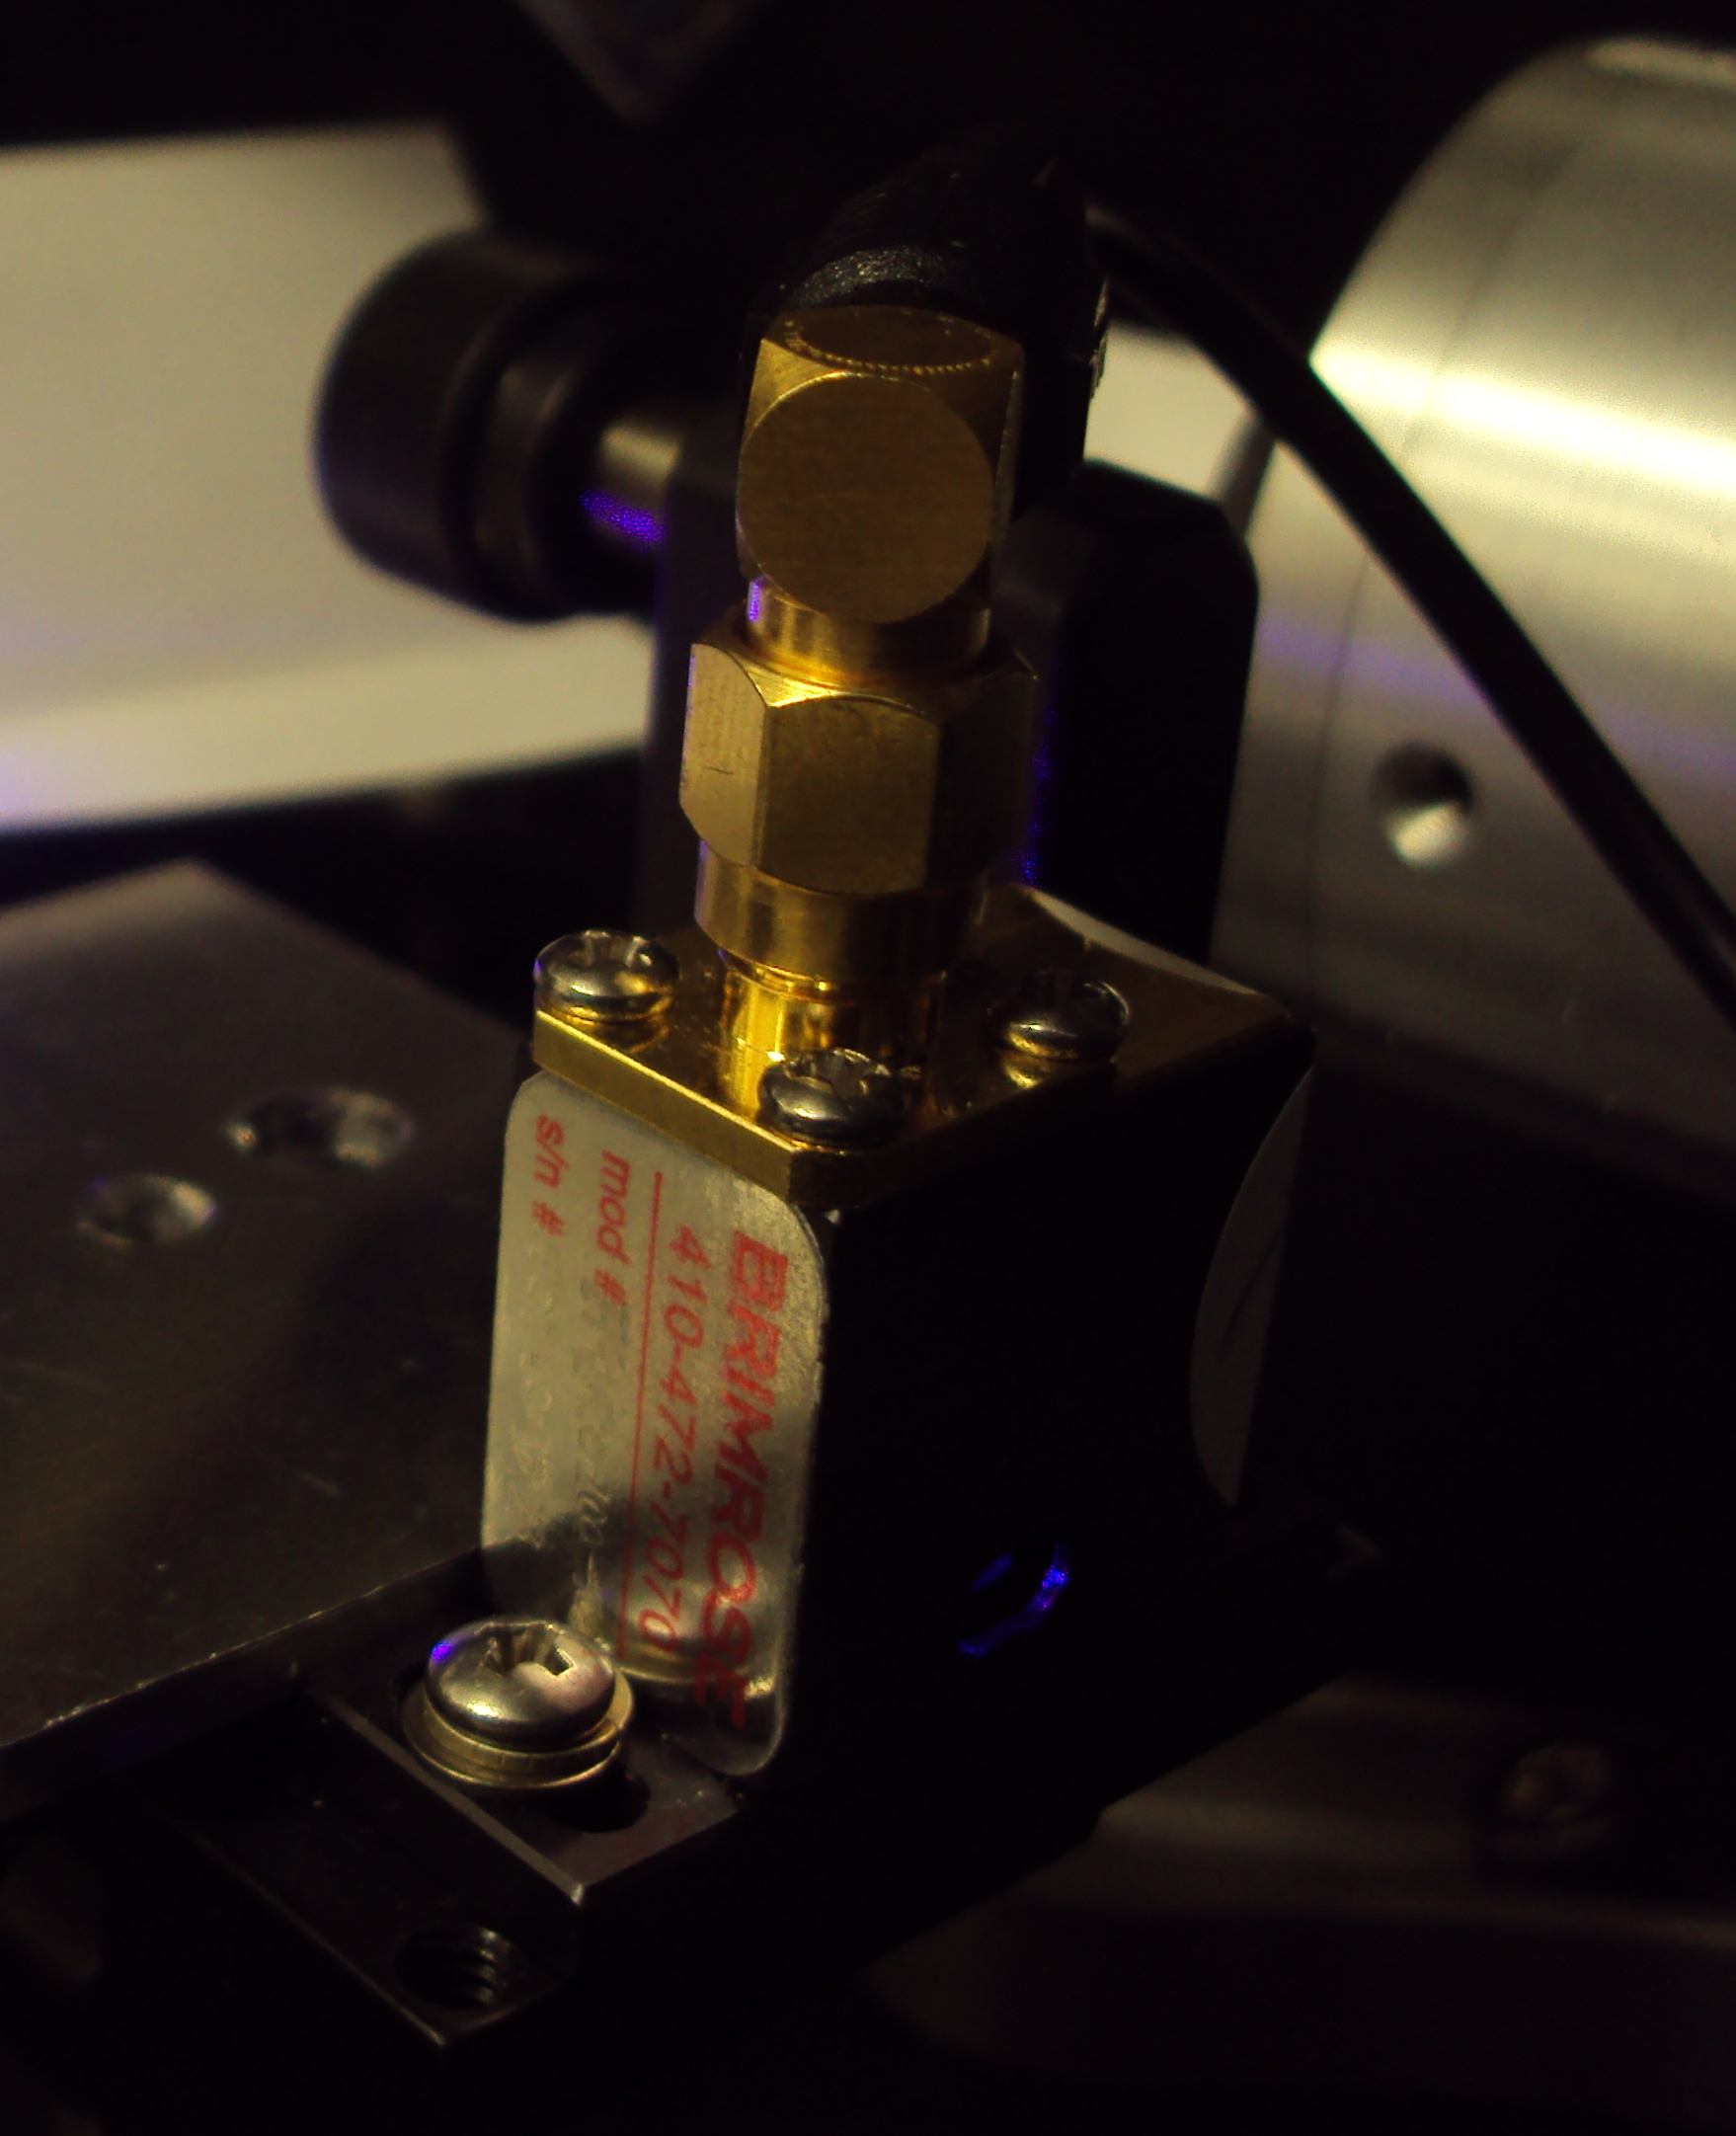
\includegraphics[width=0.95\textwidth]{aom_upclose.JPG}}
\caption[Photograph of AOM]{\label{aom_upclose} The AOM mounted in the setup. The aluminum plate in the lower left part of the photo that can be seen butting up against the AOM was used only as a guide for initial AOM alignment and was removed in the final system.}
\end{figure}
\begin{figure}
\centerline{
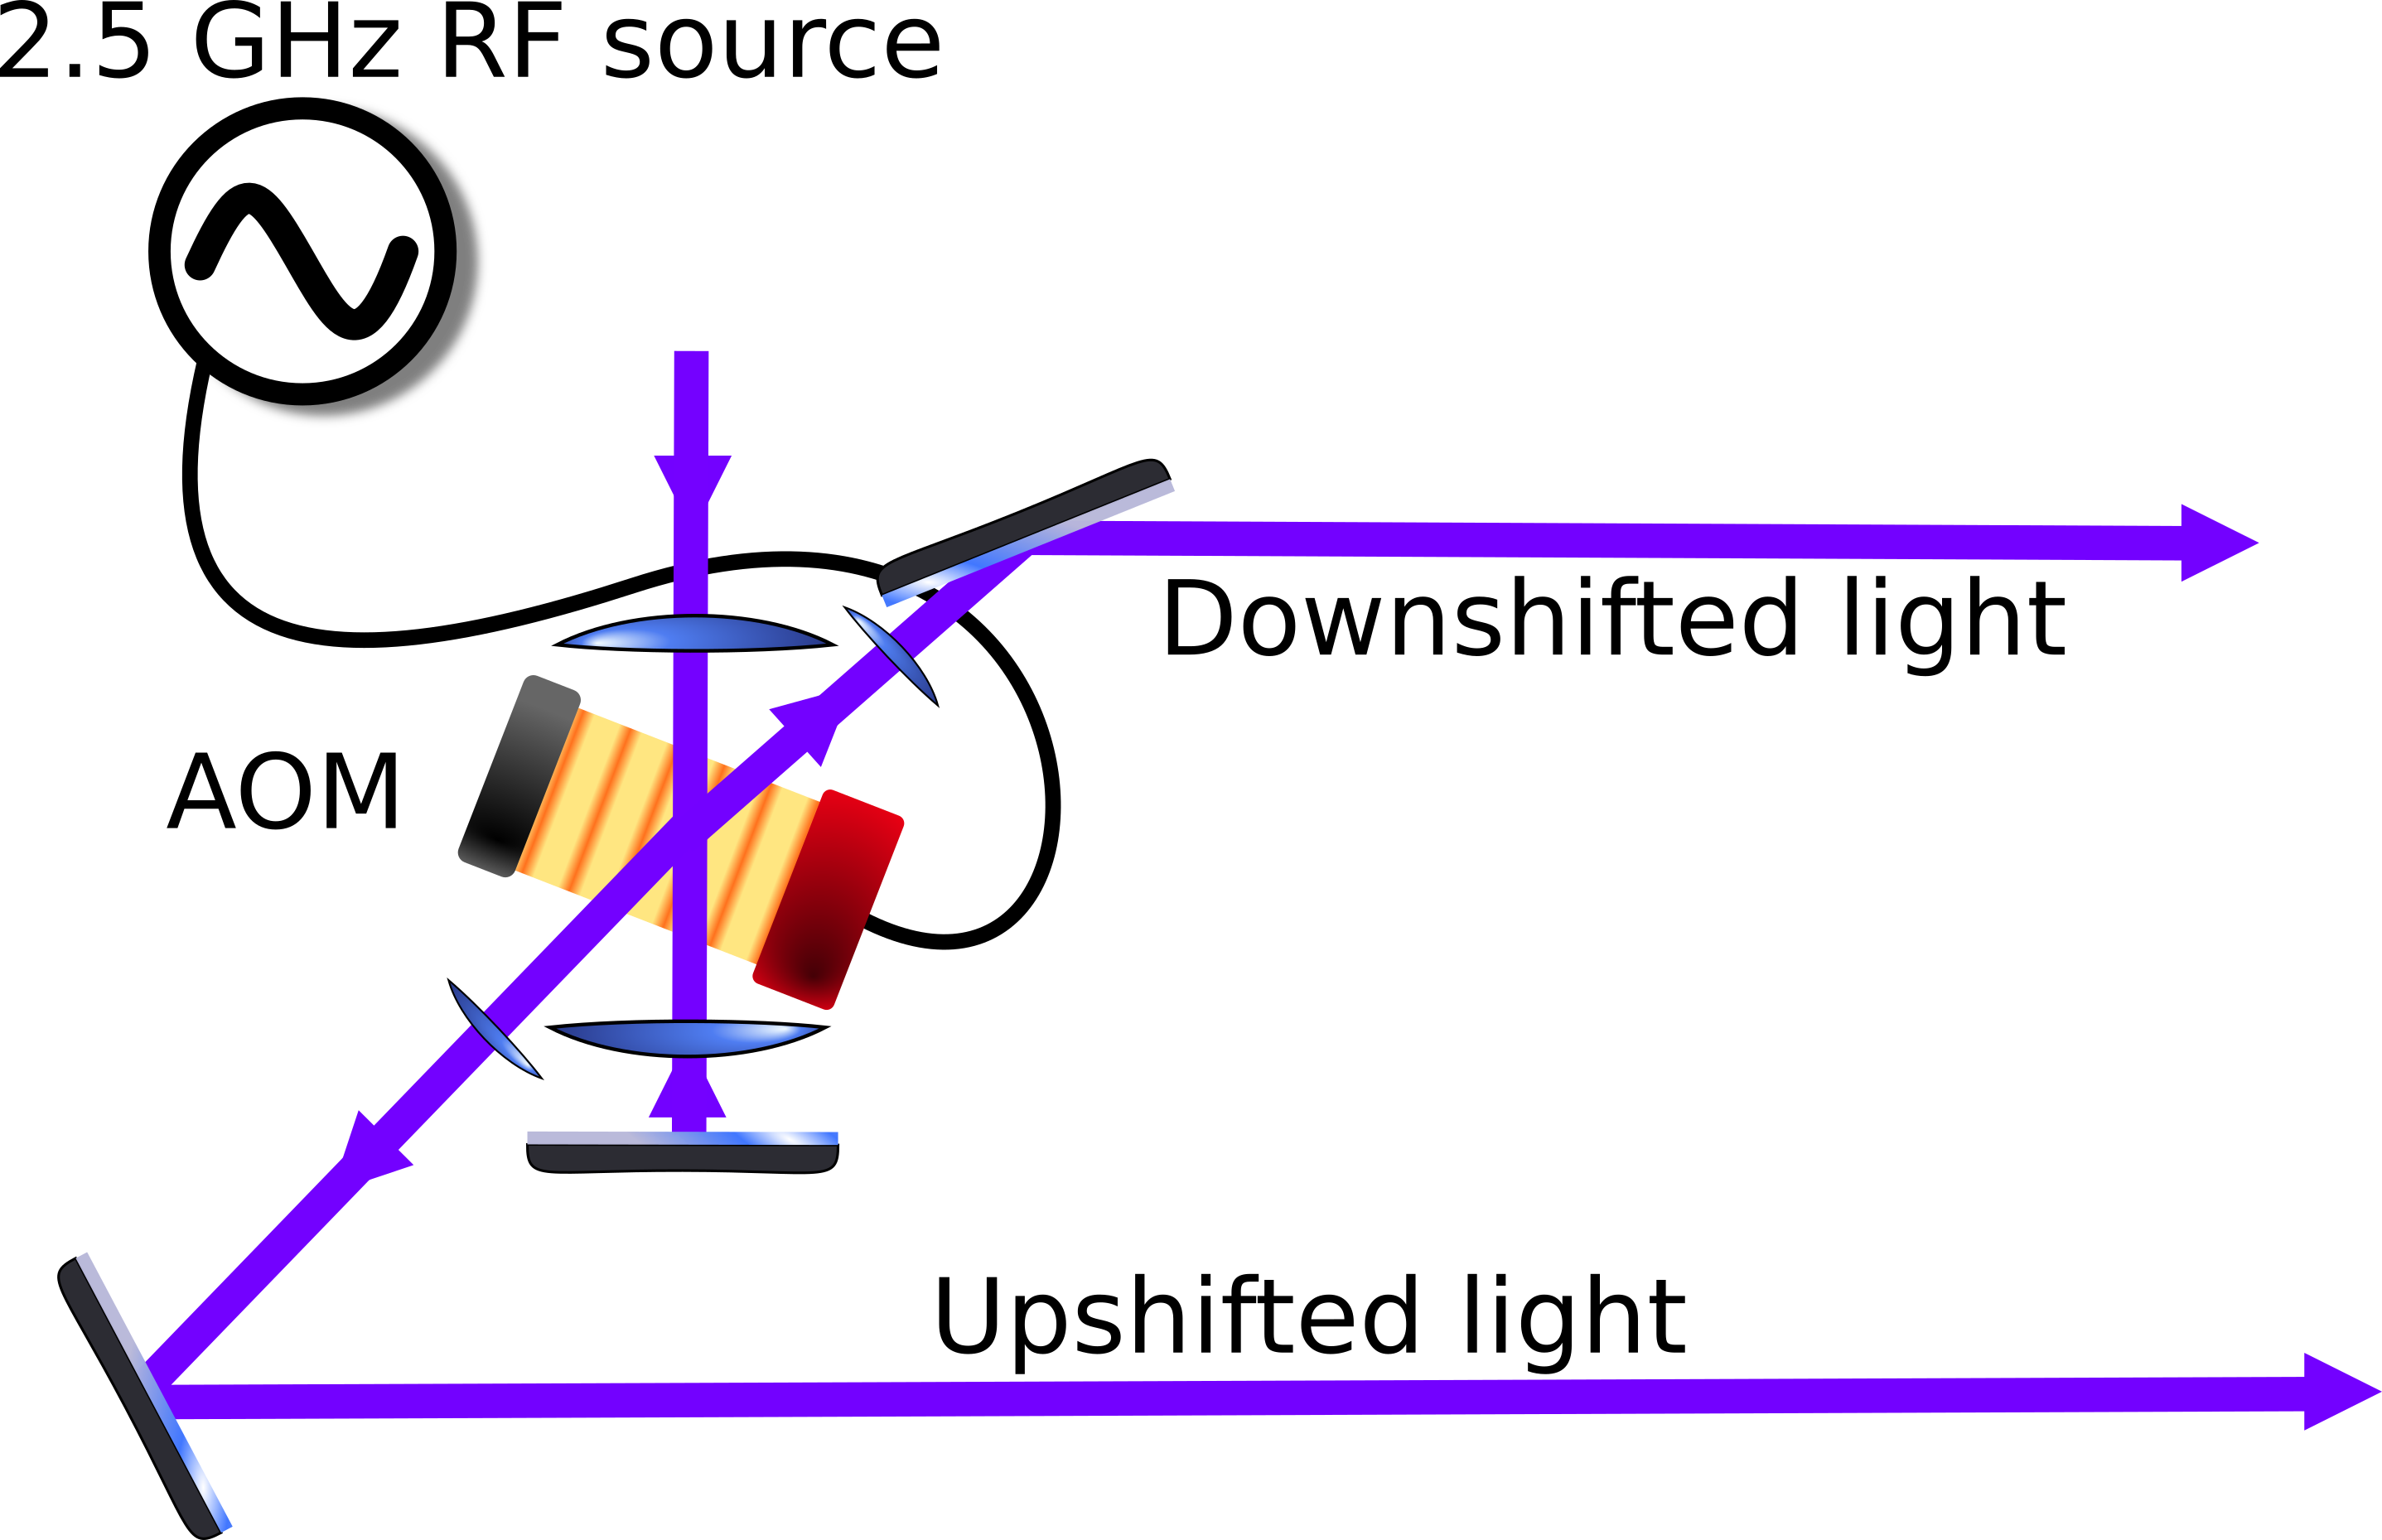
\includegraphics[width=0.95\textwidth]{diagramOfAOM}}
\caption[AOM diagram]{\label{aomDiagramDetail} Detail of Figure\,\ref{figdiagramOfSetup}. The light from the master laser is depicted entering from the top of the diagram. This beam travels into the AOM, which is depicted in the center of the diagram. The red shifted light is depicted travelling towards the lens and mirror near the lower left side of the diagram. The zeroth order diffracted beam is recollimated and then retroreflected. The blue shifted light is depicted exiting the AOM towards the top right of the figure.}
\end{figure}

The AOM we used was a TEF-2500-200-405 made by Brimrose Corporation of America. The crystal material was Tellurium Flouride, the center carrier frequency is 2500 MHz, the bandwidth (3dB) was 200 MHz. The AOM's anti-reflective coatings are specified to work at 405 nm. 
\section{Principle of Operation}

The AOM is a crystal with a piezoelectric transducer attached to one side and an acoustic absorber attached to the other side. Acoustic waves are produced by the tranducer. These waves travel across the active area of the AOM crystal and are absorbed by the absorber on the other side. The compression and decompression caused by the travelling acoustic waves changes the index of refraction within the crystal and because of this, the light can experience Bragg reflection off the acoustic wavefronts. Because the effective reflective surface is moving, the light scattered off these features is Doppler-shifted and emerges at a distinct angle compared to the incoming light. This allows the AOM to produce frequency-shifted beams. 

The calculation of the frequency shift and Bragg angle of an AOM are well-known. The relationship between the driving frequency and the Bragg angle is 


\begin{equation}
\sin{\theta}=\frac{m \lambda}{2 \Lambda}
\end{equation}

The relationship between the driving frequency and the shift in the frequency of the light simply turns out to be 

\begin{equation}
    f_{\textnormal{driving}}=\Delta f_{\textnormal{laser}}.
\end{equation}

Ultimately, getting the AOM to work properly involves optimizing just a few parameters. We must ensure that the AOM is installed at the right angle relative to the incoming beam. We must ensure that as much of the incoming beam as possible hits the active area of the AOM. This requires alignment in the X and Y dimensions, but it also means that we attempt to maneuver the AOM so that the focal point of the incoming beam is approximately in the center of the crystal. The power used to drive the piezoelectric transducer must be optimized. Furthermore, the intensity and shape of the incoming beam must be adjusted to ensure that we do not exceed the maximum allowable intensity for the AOM, which is specified as 50 W/mm$^2$.
%shape instead of waist?
Thus, we will first discuss some work we did to characterize our incoming beam.

\section{Optimization of Beam Waist}
First, we would like to control our beam so that, at its focus, the majority of the beam fits within the active area of the AOM 
%\footnote{I did explore the possibility of just sending in a huge beam with lots of extra power in hopes that the part scattering off the active part of the AOM would work. Preliminary tests showed little promise for the technique. Furthermore, we would expect the possibility of severe distortion of the transverse mode of our laser.}
This area is specified as being .05 mm wide. 

Our goal is to have a beam waist radius that will be $\approx$4 times smaller than this 0.05 mm value\footnote{Note I am comparing the beam waist \emph{radius} to the \emph{width} of the active area.}. If our waist is too small, we have to reduce the power to avoid damaging the AOM. Also, the diffraction efficiency decreases because the beam will interact with fewer Bragg planes. If the waist is too large, only a small portion of the beam would be within the active area of the AOM and would thus possibly suffer distortion of its transverse mode. A beam that is focused to too large a size would also reflect less light.

We can model the laser as a Gaussian beam. Gaussian beams have the property that their intensity profile always takes a Gaussian shape, i.e. \cite{lasersMilonniEberly}
\begin{equation}
    I(\mathbf{r})=I_0\exp{-2(r^2/w(z)^2)}
\end{equation}

The waist of a Gaussian Beam is given by:

\begin{equation}
    w(z)=\sqrt{s+\frac{z^2}{z_0^2}}
\end{equation}

where $w(z)$ is the distance from the center of the beam to the point where the intensity of the beam has fallen by a factor of $1/e^2$ (i.e. the spot size), $z$ is the distance along the direction of propagation between the beam waist and the plane where we are evaluating $w(z)$ and $z0$ is the Rayleigh range, which also satisfies the relation 

\begin{equation}
    z_0=\pi w_0^2/\lambda
\end{equation}

A slight modification of this allows us to model elliptical beams by allowing for a different waist in each of the $x$ and $y$ directions:

\begin{equation}\label{eqForI}
    I(\mathbf{x,y})=I_0\exp{-2(x^2/w_x(z)^2+(y^2/w_y(z)^2))}
\end{equation}

We can measure the beam-waist radius using a standard knife-edge technique. This involves placing a photodiode in the path of the beam.  A razor blade is then moved perpendicular to the beam in a controlled way such that the beam is partially blocked. For each razor blade position, we measure the power incident on the photodiode. By integrating Eq.\,\ref{eqForI}, we get

\begin{equation}
{\rm Power\ incident\ on\ photodiode}=\frac{1}{2} P \left(\erf \left( \frac{\sqrt{2} x}{W_{0x}}\right)\right)
\end{equation}
%get data for this?
We do this several times at various points along the path of the laser and can perform a curve fit to calculate our beam divergence and therefore infer its waist.

We were somewhat worried that modeling our beam as a Gaussian would not be adequate. This was in part due to irregularities in the transverse mode of the master laser \footnote{The experiment still worked -- all that matters is that we are able to get the master laser stable and couple diffracted light from the AOM into the slave lasers. Ultimately, it was discovered by other students that this was due to a manufacturing defect in the optical isolators.} Because we were planning to operate the AOM relatively close to its damage threshold, we examined the possibility of using a more sophisticated theory to model our beam based on measurable parameters. 

Siegman \cite{SiegmanBeamQuality} discusses the characterization of beams in terms of a quantity that is known simply as ``$M^2$.'' $M^2$ is a measure of how Gaussian a beam is. If a beam is Gaussian, $M^2=1$. If a beam contains higher order Laguerre-Gaussian modes, $M^2$ will be greater than 1. Ref.\,\cite{SiegmanBeamQuality} demonstrates that any beam comprised of Laguerre-Gaussian modes can be mathematically proven to propagate according to the following equation:

\begin{equation}
\sigma_x^2=\sigma_{0x}^2+\left( \frac{M_x^2 \,\lambda}{\pi \, \sigma_{0x}}\right)^2 (z-z_{0x})^2 \label{SiegmanBeamPropagate00}
\end{equation}
where $\sigma_x^2$ (or second-moment width) is given by 
\begin{equation}\label{secondMomentWidth}
\sigma_x^2=\frac{\int_{-\infty}^{\infty} (x-x_0)^2 I(x,y)\, dx\, dy}{\int_{-\infty}^{\infty} I(x,y)\, dx \, dy}
\end{equation} 
where $I(x,y)$ is the intensity profile of our beam, which is propagating in the $z$ direction. In the special case of the Gaussian beam, $2\sigma_x=w_x$.

In principle, we could take measurements of $\sigma_x^2$ our beam using the knife edge technique described above at several points along the beam's path and then fit this to Eq.\,\ref{SiegmanBeamPropagate00}.
We tried allowing $M^2$ to be one of our fit parameters as we analyzed data from our beam, but we found it difficult to get data of sufficient quality to give a good estimate. The knife edge data is hard to get with sufficient resolution over a large enough range. One problem is that the contribution to $\sigma_x$ increases as the square of the distance from the center of the beam. This means that we have to have very accurate measurements of our background offset. We also attempted to use a camera, but were not able to trust its linearity and offsets enough to get good results. Information about our attempt to calibrate the camera can be found in Appendix\,\ref{BeamWaistAppendix}. 

However, we did consider what implications it would have for our beam if $M^2\neq 1$. We can look at the effective slope of divergence by rearranging Eq.\ \ref{SiegmanBeamPropagate00} and taking the limit as $(z-z_0) \rightarrow \infty$
\begin{equation}
\frac{\sigma_x}{z-z_0}=M_x^2 \frac{\lambda \pi}{\sigma_{0x}} \label{SiegmanBeamSlope}
\end{equation}
%does z0 matter as a fit parameter? I don't think so. 
Note that the smallest possible beam waist radius corresponding to any given beam divergence, occurs if $M^2=1$. Thus, if we measure the beam divergence perform our calculations for the case where $M^2=1$, we end up with a minimum calculated beam-waist radius, which corresponds to a maximum peak intensity at the center of the beam. This is effectively a ``worst case scenario.'' We can thus guarantee that the peak intensity at the focus of our beam will be less than or equal to the result of this calculation no matter what the real-life value $M^2$ actually ends up being. 


\subsection{Ray Transfer Matrix Analysis of System}
It is crucially important that we not put too much intensity through the AOM. As a sanity check, we can calculate using an ABCD matrix (ray-transfer matrix) what the beam waist should be for our optical setup. This model can be used to estimate our sensitivity to small changes in the setup. So, for example, if the collimating lens on our laser diode was not properly in place.

%This is in a lab notebook somewhere. You need to find it there, I think. Or it's in a Mathematica file. 
%found: the Mathematica files are generalABCDfinding.nb, ABCDwillWeBreakAOM.nb . The m files, well, I think the ones I want are in checkTheWaists_realDATA. 

We will model our beam using the well-known rule for modelling the change of a Gaussian beam as it passes through a system described by ray transfer matrix with coefficients $A$,$B$,$C$ and $D$, which is 

\begin{equation} \label{ABCDlawforGaussianBeams}
z'-iz_0'=\frac{A(z-iz_0)+B}{C(z-iz_0)+D}
\end{equation}
\cite{BYUOpticsBook}

which can be solved to give 

\begin{align}
z_0' &= \frac{ z_0 (BC-AD)}{C^2z^2+C^2z_0^2+2 C D z + D^2} \\
z' &=\frac{AC z^2+ACz_0^2+ADz+BCz+BD}{C^2z^2+C^2z_0^2+2 C D z + D^2}
\end{align}

This calculation should give us a feel for how sensitive we are to drifts in the optical setup. We will also be able to verify that the beam waist near the AOM is close to what we would expect based on the beam waist at the laser diode.

The system has only a few components that we need to model. At the start, we assume that the light coming out of the face of the laser diode is essentially a Gaussian beam with different beam waist radii for the $x$ and $y$ directions. We see in the datasheet that a typical angle of divergence for light coming out of one of these lasers is going to be 9$^\circ$ and 19$^\circ$. A Gaussian beam's angular divergence can be surmised by looking at Eq.\ \ref{SiegmanBeamSlope}. The relationship turns out to be \cite{MellesGriotGaussian}. One can use the given angle of divergence of light from the laser diode in order to infer what the equivalent Gaussian beam radii are. These turn out to be 972.913 nm and 460.854 nm. 

The light from the laser head is emitted and collimated by a lens\footnote{Thorlabs C570TM-A} with focal point 2.84 mm.%before, I had 2.87 mm, IDK why
The beam goes through various components whose collective impact can be modeled as simple propagation over some effective distance. Even though propagating through a medium like the crystals in our isolators is different than propagating through air, travelling some distance through any medium is the same as travelling some effective distance through air. Since we can't measure the total path length very accurately anyway, we just fold the propagation through these crystals into the overall propagation.
We estimate the the effective distanceo of propagation should be on the order of 1 m. The beam is then focused by a lens with focal length 10 cm and passed through the AOM. 

We can write the ABCD matrix for the whole system as the following product of ABCD matrices: 

\begin{equation}\label{ABCDMatrixSystem}
\begin{bmatrix}
1 & 0 \\ -1/f_{f} & 1
\end{bmatrix}
\begin{bmatrix}
1 & d_2-d_1 \\ 0 & 1
\end{bmatrix}
\begin{bmatrix}
1 & 0 \\ -1/f_{a} & 1
\end{bmatrix}
\begin{bmatrix}
1 & d_1 \\ 0 & 1
\end{bmatrix}
=
\begin{bmatrix}
A & B \\ C & D
\end{bmatrix}
\end{equation}

Finding the resulting ray transfer matrix that describes the system involves simply performing the matrix multiplication prescribed in Eq.\,\ref{ABCDMatrixSystem}. However, we opt not to write out result in this thesis. Instead, we used Mathematica to find the expressions for $z_0'$ and $z'$. These expressions were then evaluated numerically for several values of likely experimental parameters. In particular, we were interested in verifying that the beam waist inside the AOM remains reasonable for realistic values of $d_1$ (the distance from the laser face to the collimating lens) and $d_2$ (the distance traveled between the collimating lens and the other lens), since these are values that may change in the future.

From this analysis, we calculate the effective area of our beam and the corresponding ratio between the intensity at the most intense part of the beam and the total power in the beam. If we see that these ratios do not change too much for reasonable parameters, we need not fear that a slight change in the position of one of our optical elements will be disastrous:

\begin{figure}
    %\centerline{\includegraphics[trim=100pt 100pt 100pt 100pt, clip=true, totalheight=0.5\textheight,angle=90]{testfigure}}
    %\centerline{\includegraphics[totalheight=0.3\textheight]{testfigure}}
    \centerline{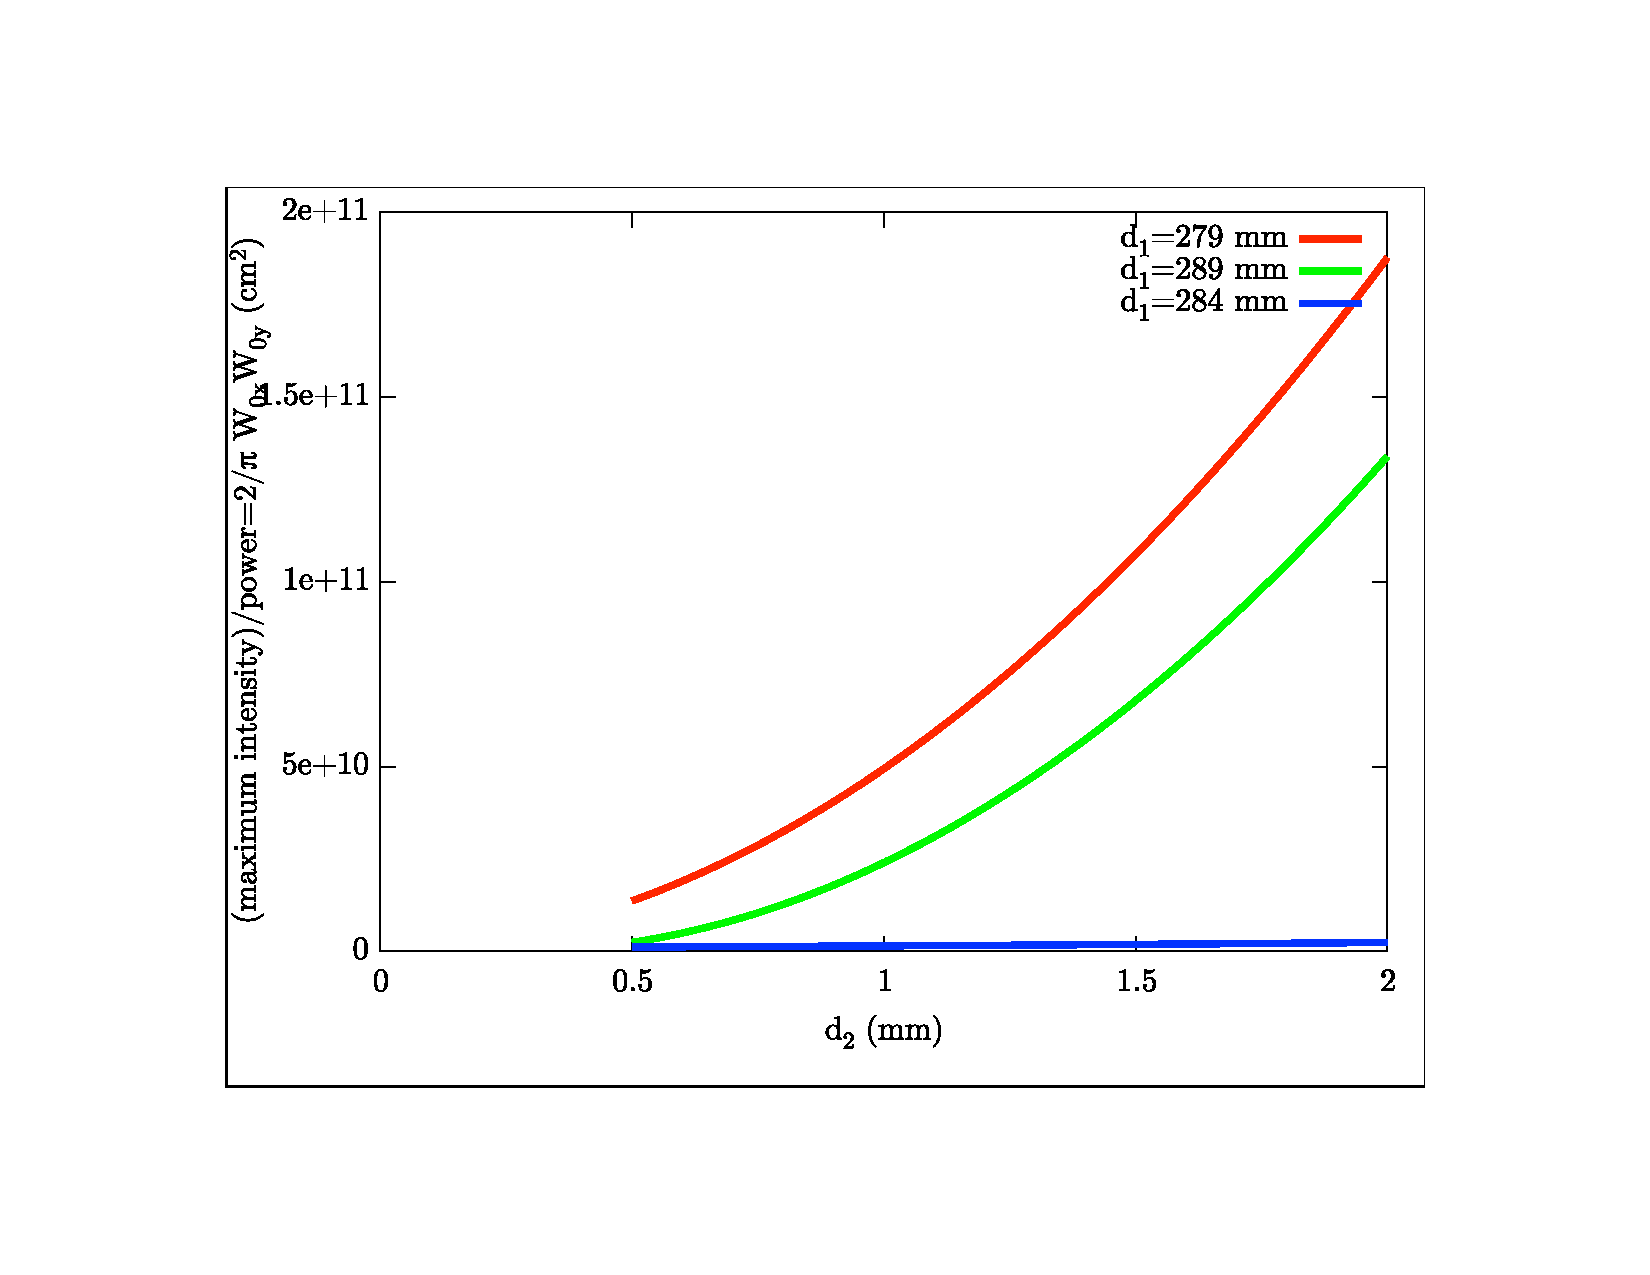
\includegraphics{waists1}}
    %\includegraphics[totalheight=0.3\textheight]{testfigure}
    \caption[]{\label{waists1} The ratio of the maximum intensity to the total beam power as a function of the distance between the laser's collimating lens and the focusing lens ($d_2$) plotted for several values of $d_1$, which is the distance between the laser diode's output face and the collimating lens.}
\end{figure}

\begin{figure}
    %\centerline{\includegraphics[trim=100pt 100pt 100pt 100pt, clip=true, totalheight=0.5\textheight,angle=90]{testfigure}}
    %\centerline{\includegraphics[totalheight=0.3\textheight]{testfigure}}
    \centerline{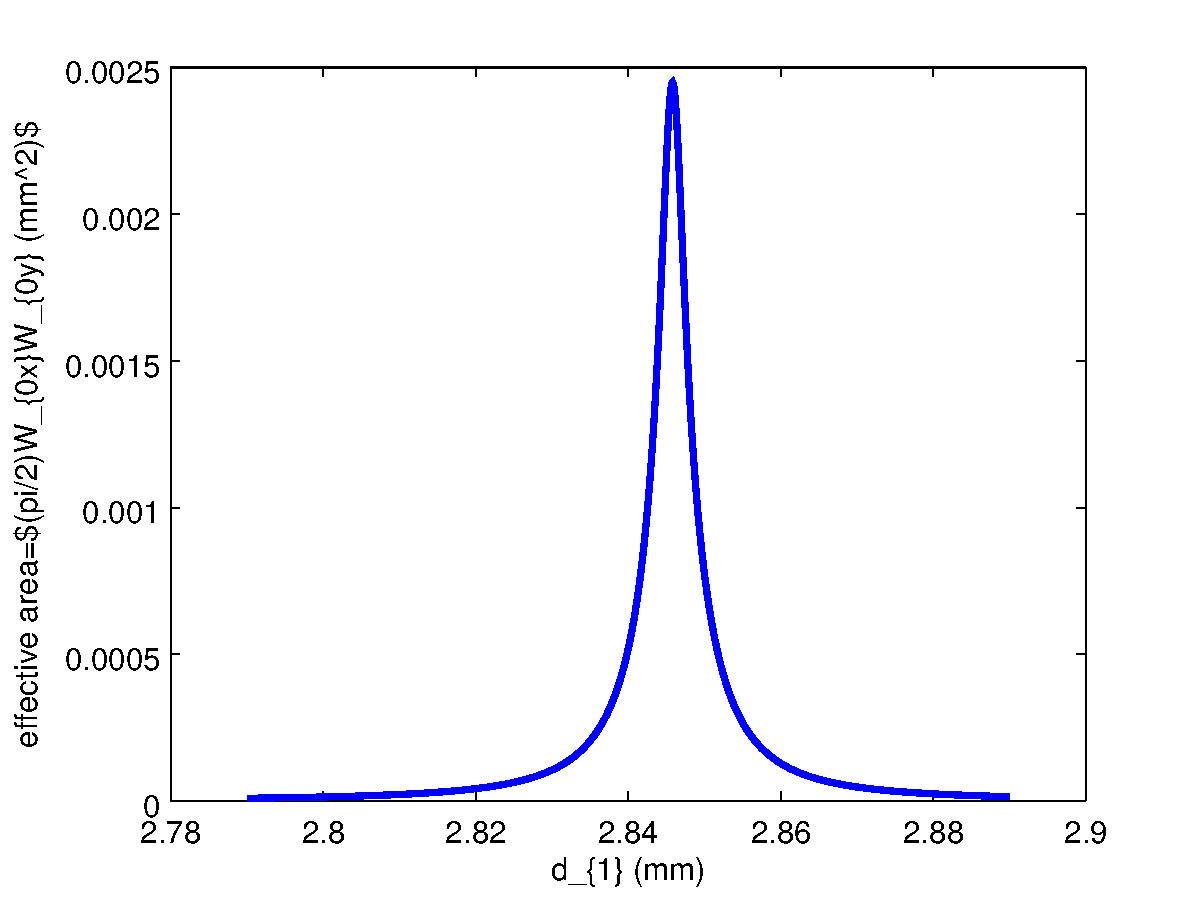
\includegraphics{waists2}}
    %\includegraphics[totalheight=0.3\textheight]{testfigure}
    \caption[]{\label{waists2}
        The effective beam area as a function of the distance between the laser diode's output face and the collimating lens ($d_1$).}
\end{figure}
